%# -*- coding:utf-8 -*-
\documentclass[10pt,aspectratio=43,mathserif]{beamer}		
%设置为 Beamer 文档类型,设置字体为 10pt,长宽比为4:3,数学字体为 serif 风格

%%%%-----导入宏包-----%%%%
\usepackage{scnu}			%导入 SCNU 模板宏包
\usepackage[UTF8]{ctex}			%导入 ctex 宏包,添加中文支持,指定 UTF8 编码
\usepackage{amsmath,amsfonts,amssymb,bm}   %导入数学公式所需宏包
\usepackage{color}			 %字体颜色支持
\usepackage{graphicx,url}
\usepackage{listings}

\usepackage[
	n, 
	operators, 
	advantage, 
	sets, 
	adversary, 
	landau, 
	probability, 
	notions, 	
	logic, 
	ff, 
	mm, 
	primitives, 
	events, 
	complexity, 
	asymptotics, 
	keys]{cryptocode}

% 设置中文字体 (如果需要)

\setCJKmainfont{Source Han Sans SC VF}
\setCJKsansfont{Source Han Serif SC}
\setCJKmonofont{Source Han Serif SC}

\beamertemplateballitem		%设置 Beamer 主题

%%%%------------------------%%%%%
\catcode`\。=\active         %或者=13
\newcommand{。}{.}				
%将正文中的"。"号转换为"."。中文标点国家规范建议科技文献中的句号用圆点替代
%%%%%%%%%%%%%%%%%%%%%

%%%%----首页信息设置----%%%%
\title[多阶段密钥交换协议]{一种多阶段密钥交换协议的设计与实现}
\subtitle{}		
%%%%----标题设置


\author[史豪]{
  答辩人:史豪 \\\medskip
  指导老师:王立斌}
%%%%----个人信息设置

\institute[华南师范大学]{
  华南师范大学
}
%%%%----机构信息

\date[2025年4月]{
  2025年4月28日}
%%%%----日期信息
  
\begin{document}

\begin{frame}
\titlepage
\end{frame}				%生成标题页

\section{}
\begin{frame}
\frametitle{目录}
\tableofcontents
\end{frame}				%生成提纲页

\section{研究目标}
\begin{frame}
\frametitle{研究目标}

\begin{itemize}
    \item 量子计算威胁传统密码体系
    \item 多阶段密钥交换 (MSKE) 协议在现代网络通信的广泛应用
    \item TIMKE 协议提供紧致安全和后量子安全,有望解决大规模部署的安全问题
\end{itemize}
\end{frame}

% TODO 介绍多阶段,展示TIMKE的协议

\begin{frame}
\frametitle{TIMKE协议图}
\begin{center}
  \resizebox {\textwidth} {!} {
  \fbox{
  \pseudocode{%
   \textbf{客户端 $\mathbf{C}$} \< \< \textbf{服务器 $\mathbf{S}$}  \\[0.1\baselineskip][\hline]
   \<\< \\[-0.5\baselineskip]
  \text{服务器预共享的长期公钥 }\ pk_S \< \<  \text{服务器的长期私钥 }\ sk_S \\
  (\text{epk}_C, \text{esk}_C)\gets \text{Gen$_2$(par)} \< \<  \\
  {(C_1, K_{1})\gets \text{Encap$_1$}(pk_S)} \< \<  \\[-1\baselineskip]
  \< \sendmessageright{top=${\mathrm{epk}_C, C_1}$} \<  \\[-0.8\baselineskip]
  \text{K}_\text{tmp}:=\text{H}_1({pk}_S, C_1, K_1)\< \< K_{1} := \text{Decap$_1$}(sk_S, C_1) \\
  C_{payload}\gets \mathrm{Enc}(\mathrm{K_{tmp}}; M_\text{0-RTT}) \< \< \text{K}_\text{tmp}:=\text{H}_1({pk}_S, C_1, K_1)\\[-1.5\baselineskip]
  \< \sendmessageright[dotted]{top=$C_{payload}$} \<  \\[-0.4\baselineskip]
  \< \< M_\text{0-RTT}:=\text{Dec}(\text{K}_\text{tmp}, C_{payload})  \pclb [-0.5\baselineskip]\pcintertext[dotted]{Stage-1 end} \\[-1\baselineskip]
  \< \< {(C_2, K_{2})\gets \text{Encap$_2$}(\text{epk}_C)}\\[-1\baselineskip]
  \< \sendmessageleft*{C_2} \<   \\[-1\baselineskip]
  K_{2} := \text{Decap$_2$}(\text{esk}_C, C_2)\< \< \text{K}_\text{main}:=\text{H}_2(pk_S, \text{epk}_C, C_1, C_2, K_1, K_2)\\
  \text{K}_\text{main}:=\text{H}_2(pk_S, \text{epk}_C, C_1, C_2, K_1, K_2)\< \<C^\prime_{payload}\gets \mathrm{Enc}(\mathrm{K_{main}}; M_\text{1})\\[-1.5\baselineskip]
  \< \sendmessageleft[dotted]{top=$C^\prime_{payload}$} \<   \\[-0.4\baselineskip]
  M_\text{1}:=\text{Dec}(\text{K}_\text{main}, C^\prime_{payload}) \< \< \pclb [-0.5\baselineskip]\pcintertext[dotted]{Stage-2 end} \\[-2.5\baselineskip]
   }}
   }
\end{center}
\end{frame}

\section{主要工作内容}
\begin{frame}
\frametitle{主要工作内容}

\begin{itemize}
    \item 实现一种基于格的 OW-ChCCA KEM 
    \item 系统化实现紧致安全多阶段密钥交换协议 (TIMKE)
    \item 提供完整的演示系统与性能测试框架
\end{itemize}
\end{frame}

\begin{frame}
  \frametitle{开发语言——Golang}
  \begin{itemize}
    \item 提供完善的密码学支持
    \item 静态类型系统和内存安全
    \item 跨平台兼容性优秀
    \item 编译速度快 
    \item 拥有强大的并发处理能力
  \end{itemize}
\end{frame}

\section{OW-ChCCA KEM 实现}
\begin{frame}
\frametitle{OW-ChCCA KEM 实现}

\begin{itemize}
    \item 基于格的OW-ChCCA KEM 的数据结构设计、算法实现
    \item 性能优化(并行矩阵运算、优化内存管理等)
\end{itemize}
\end{frame}

\begin{frame}
\frametitle{基于格的OW-ChCCA KEM}
  \begin{figure}
    \centering
    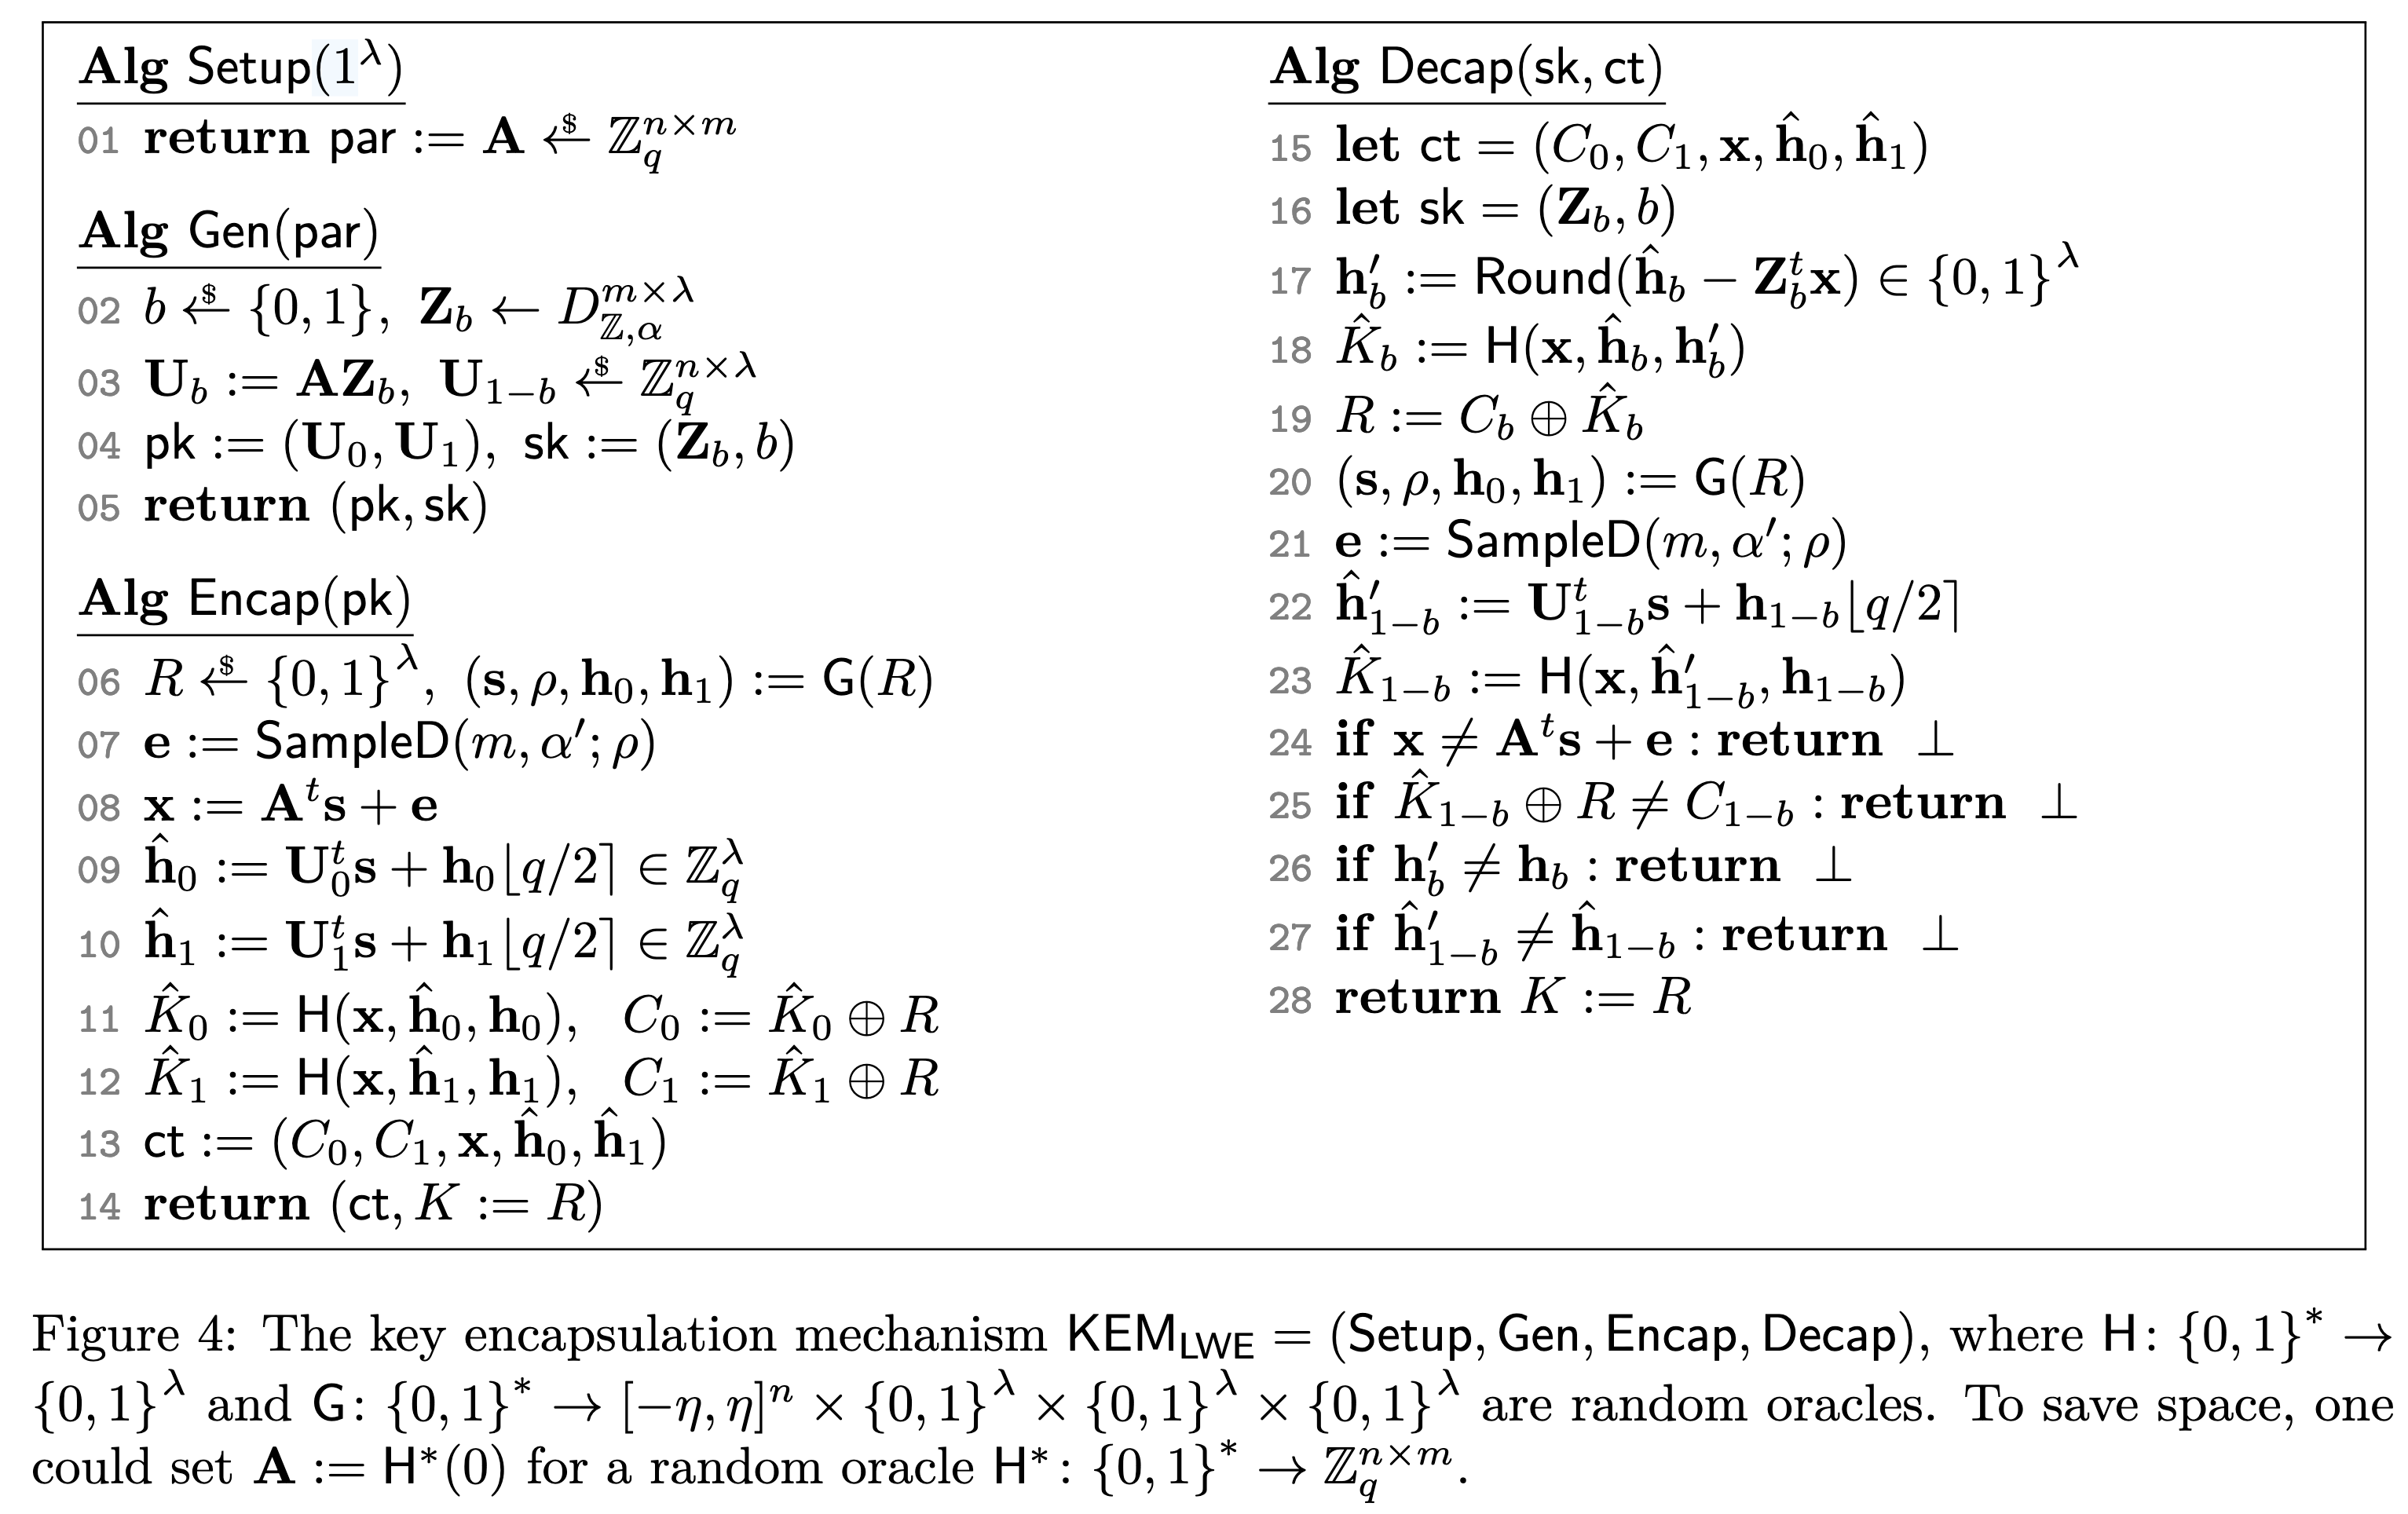
\includegraphics[width=\textwidth]{figures/owchcca.png}
  \end{figure}
\end{frame}

\section{TIMKE 协议实现}
\begin{frame}
\frametitle{TIMKE 协议实现}

\begin{itemize}
    \item 协议架构:应用层、序列化层、协议核心层、KEM 接口层、密码原语层
    \item 协议流程:预共享、第一阶段 (0-RTT)、第二阶段(弱前向安全)
\end{itemize}
\end{frame}

\begin{frame}
  \frametitle{TIMKE 协议实现 - 架构图 P.22}
 \begin{figure}
  \centering
  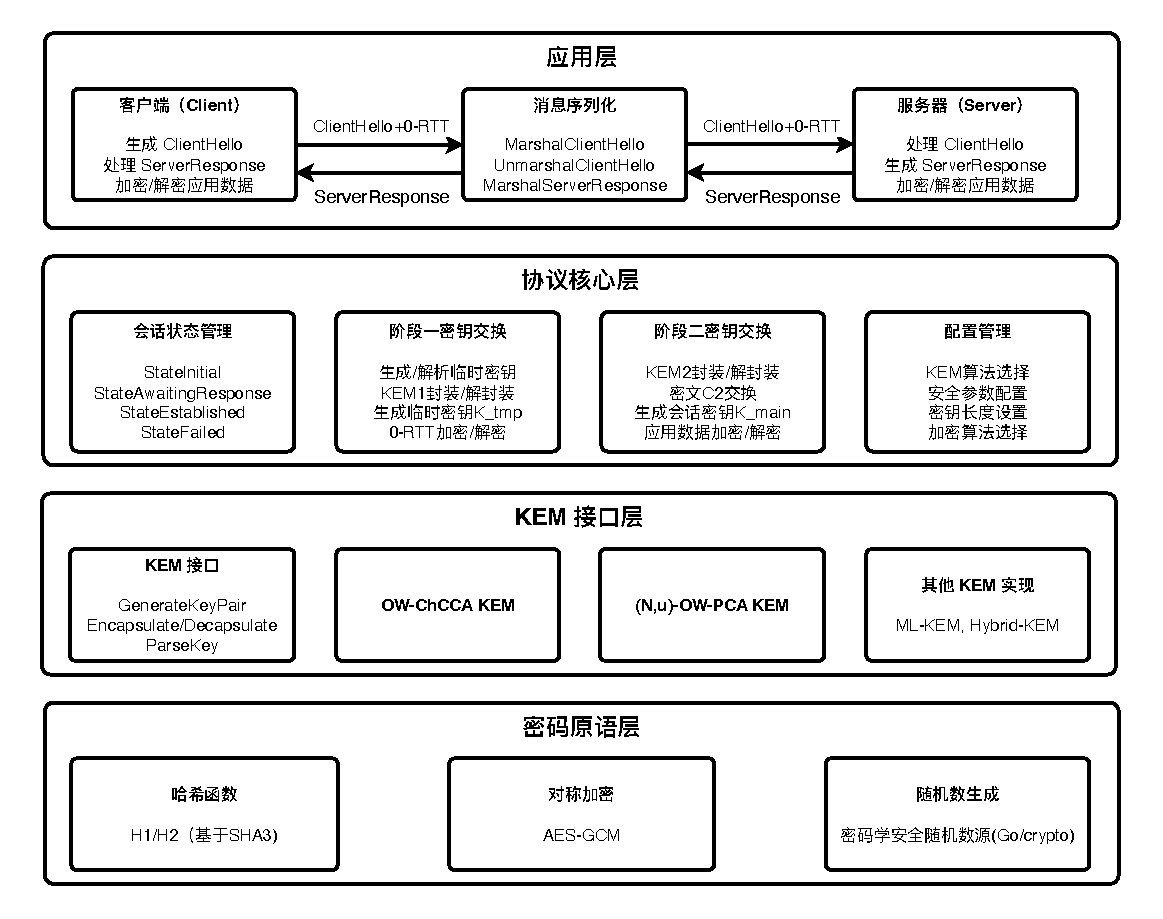
\includegraphics[width=0.8\textwidth]{figures/implementation.drawio.pdf}
 \end{figure}
\end{frame}


\begin{frame}
\frametitle{TIMKE 协议实现 - 演示系统}

\begin{figure}
    \centering
    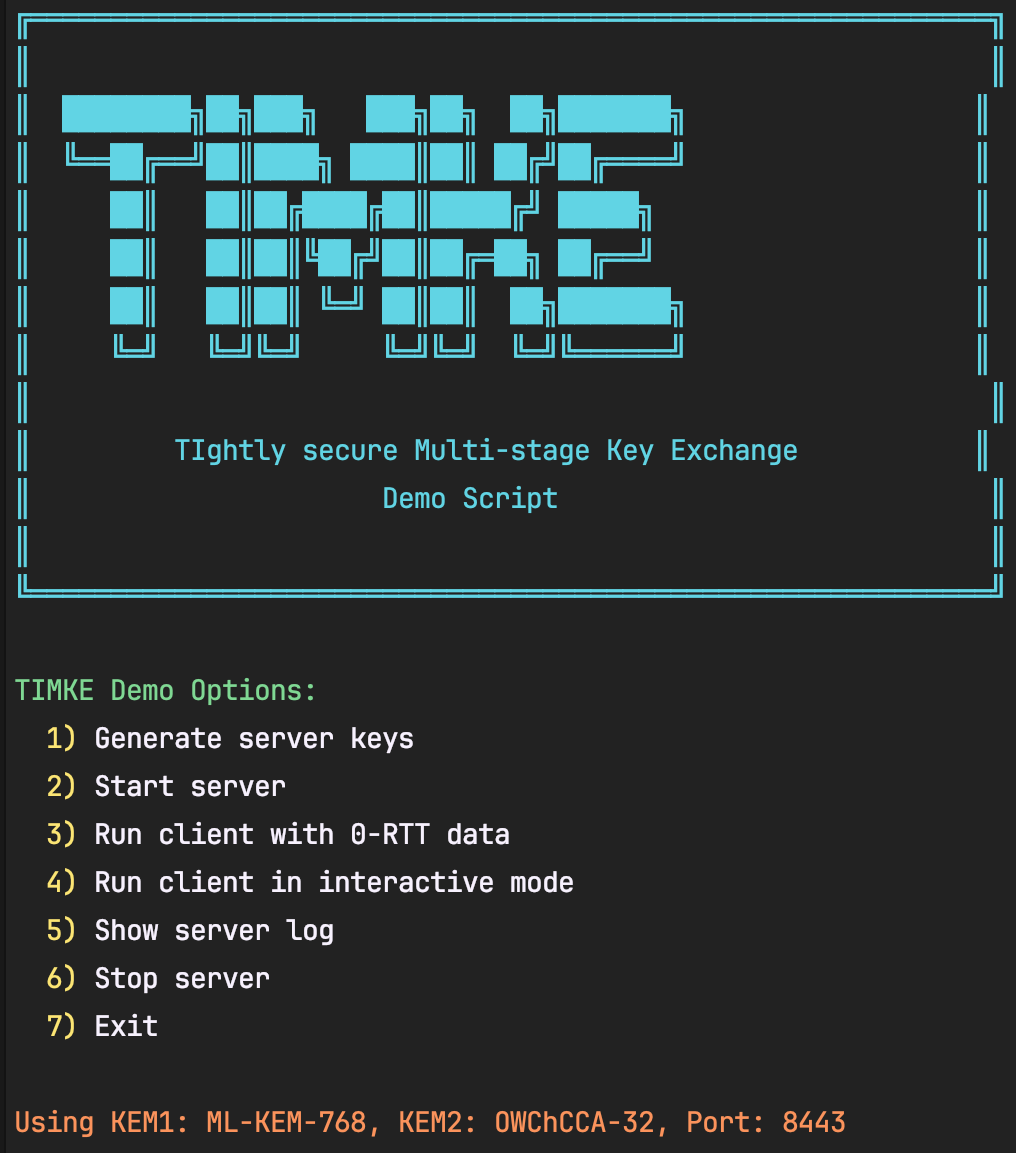
\includegraphics[width=0.5\textwidth]{figures/demo1.png}
    \caption{TIMKE 协议演示系统界面}
\end{figure}

\end{frame}

\begin{frame}
  \frametitle{TIMKE 协议实现 - 演示系统}
  
  \begin{figure}
      \centering
      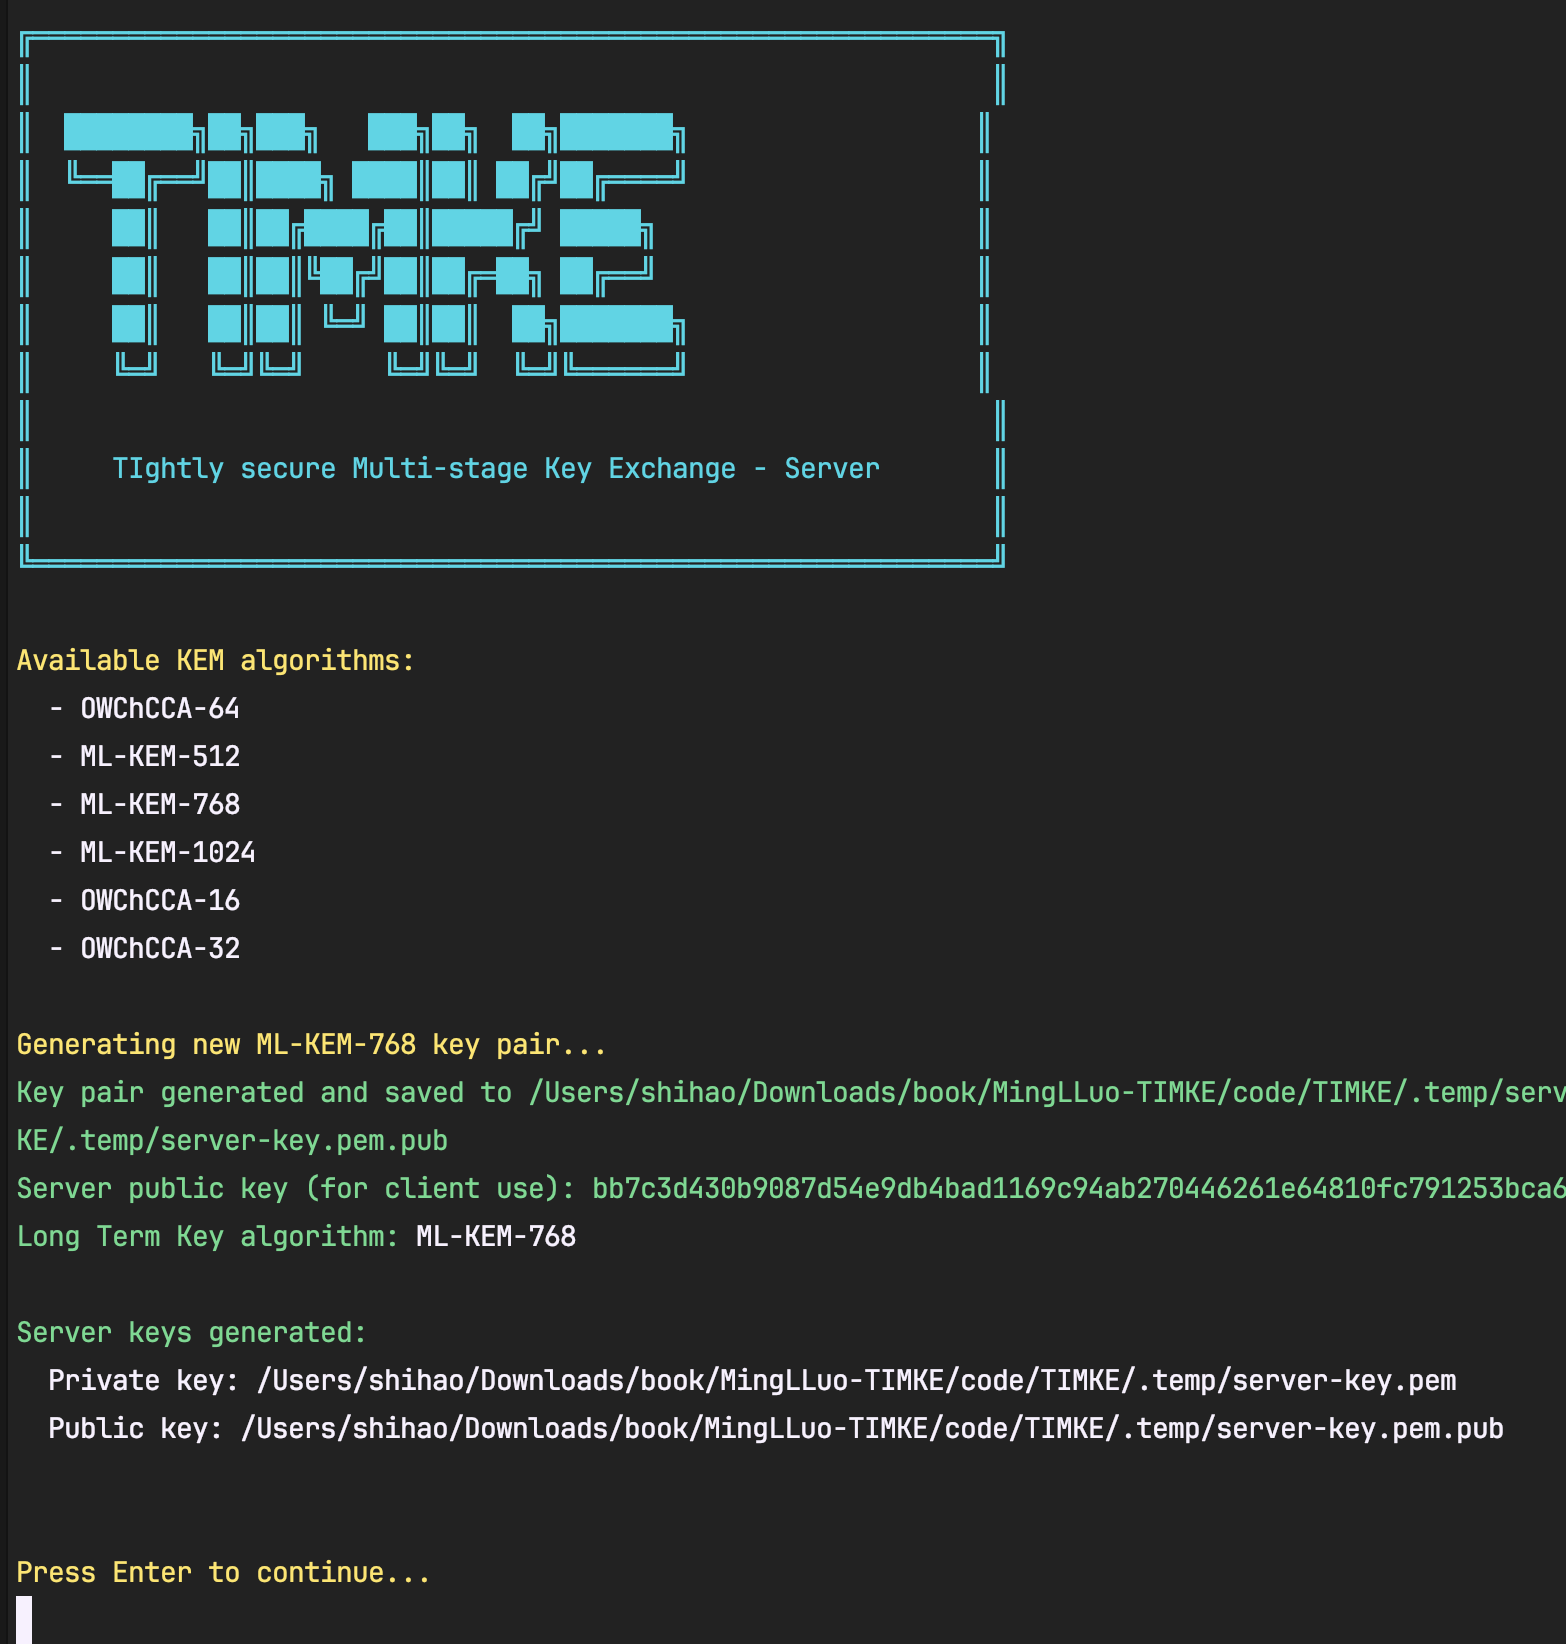
\includegraphics[width=0.5\textwidth]{figures/demo2.png}
      \caption{TIMKE 服务端长期密钥生成}
  \end{figure}
  
\end{frame}

\begin{frame}
\frametitle{TIMKE 协议实现 - 演示系统}

\begin{figure}
    \centering
    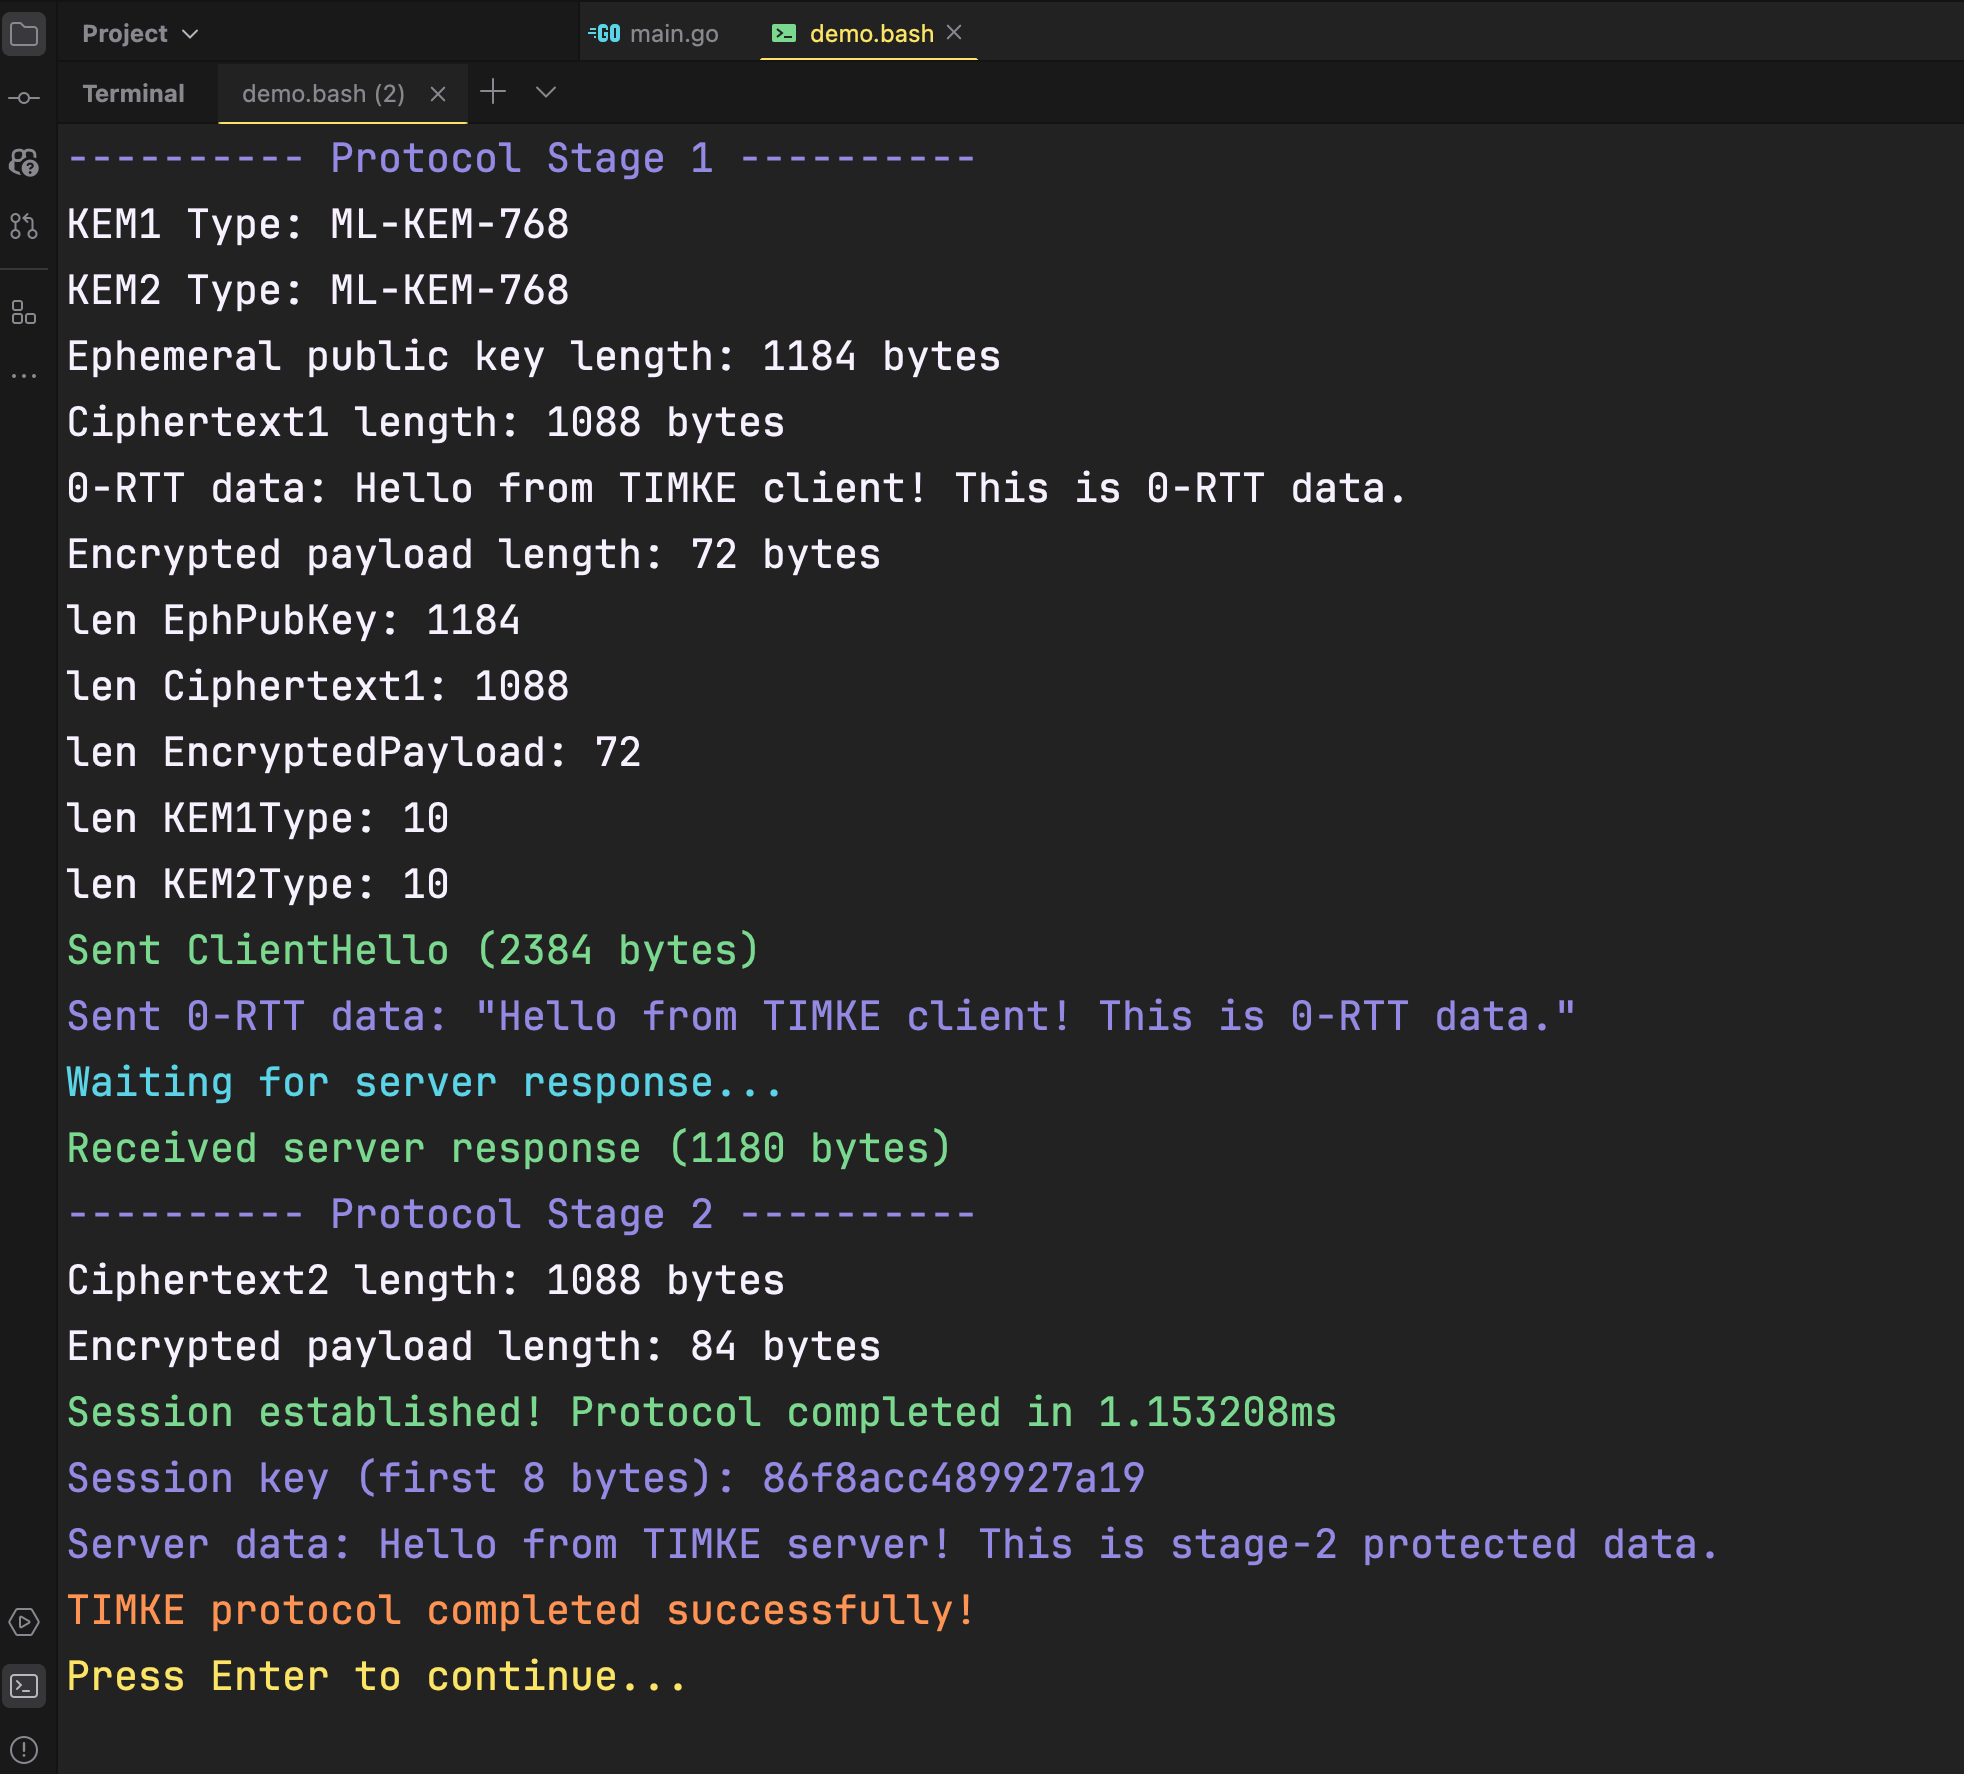
\includegraphics[width=0.6\textwidth]{figures/demo.png}
    \caption{TIMKE 协议演示系统界面}
\end{figure}

\end{frame}

\section{性能评估与分析}
\begin{frame}
\frametitle{性能评估与分析}

\begin{itemize}
    \item 评估 OW-ChCCA KEM 理论参数的实用性挑战
    \item OW-ChCCA KEM 与 ML-KEM 性能对比(计算时间、内存占用、密钥大小)
    \item 不同 KEM 组合的 TIMKE 协议性能评估
\end{itemize}
\end{frame}

\begin{frame}
\begin{table}
  \centering
  \resizebox{\textwidth}{!}{%
  \begin{tabular}{|l|r|r|r|r|}
  \hline
  \textbf{KEM组合} & \textbf{阶段1} & \textbf{阶段2} & \textbf{总时间} & \textbf{内存(KB)} \\
  \hline
  OWChCCA-mini + ML-KEM-512    & 322.18  & 118.53  & 440.71  & 2,206,372   \\
  \hline
  OWChCCA-mini + ML-KEM-768    & 324.47  & 117.61  & 442.07  & 2,206,250   \\
  \hline
  OWChCCA-mini + ML-KEM-1024   & 374.76  & 127.47  & 502.23  & 2,204,554   \\
  \hline
  \end{tabular}
  }
  \caption{混合KEM实现的TIMKE协议性能(单位:毫秒)}
\end{table}
\end{frame}


\begin{frame}
  \frametitle{性能评估与分析}
  
  \begin{itemize}
      \item 评估 OW-ChCCA KEM 理论参数的实用性挑战
      \item OW-ChCCA KEM 与 ML-KEM 性能对比(计算时间、内存占用、密钥大小)
      \item 不同 KEM 组合的 TIMKE 协议性能评估
      \item ML-KEM 替代方案的优异性能:毫秒级执行时间、低内存占用
      \item 结论:理论构造与实用性能的权衡
  \end{itemize}
  \end{frame}
\section{结论与展望}
\begin{frame}
\frametitle{结论与展望}

\begin{itemize}
    \item 主要成果:
    \begin{itemize}
        \item 实现基于格的 OW-ChCCA KEM
        \item 成功实现紧致安全后量子协议并验证其可行性
    \end{itemize}
    \item 未来工作方向:
    \begin{itemize}
        \item 结构化格上的 OW-ChCCA KEM 优化
        \item 协议功能扩展
        \item 实际应用集成
    \end{itemize}
\end{itemize}
\end{frame}

\begin{frame}
\frametitle{额外工作}

\begin{figure}
    \centering
    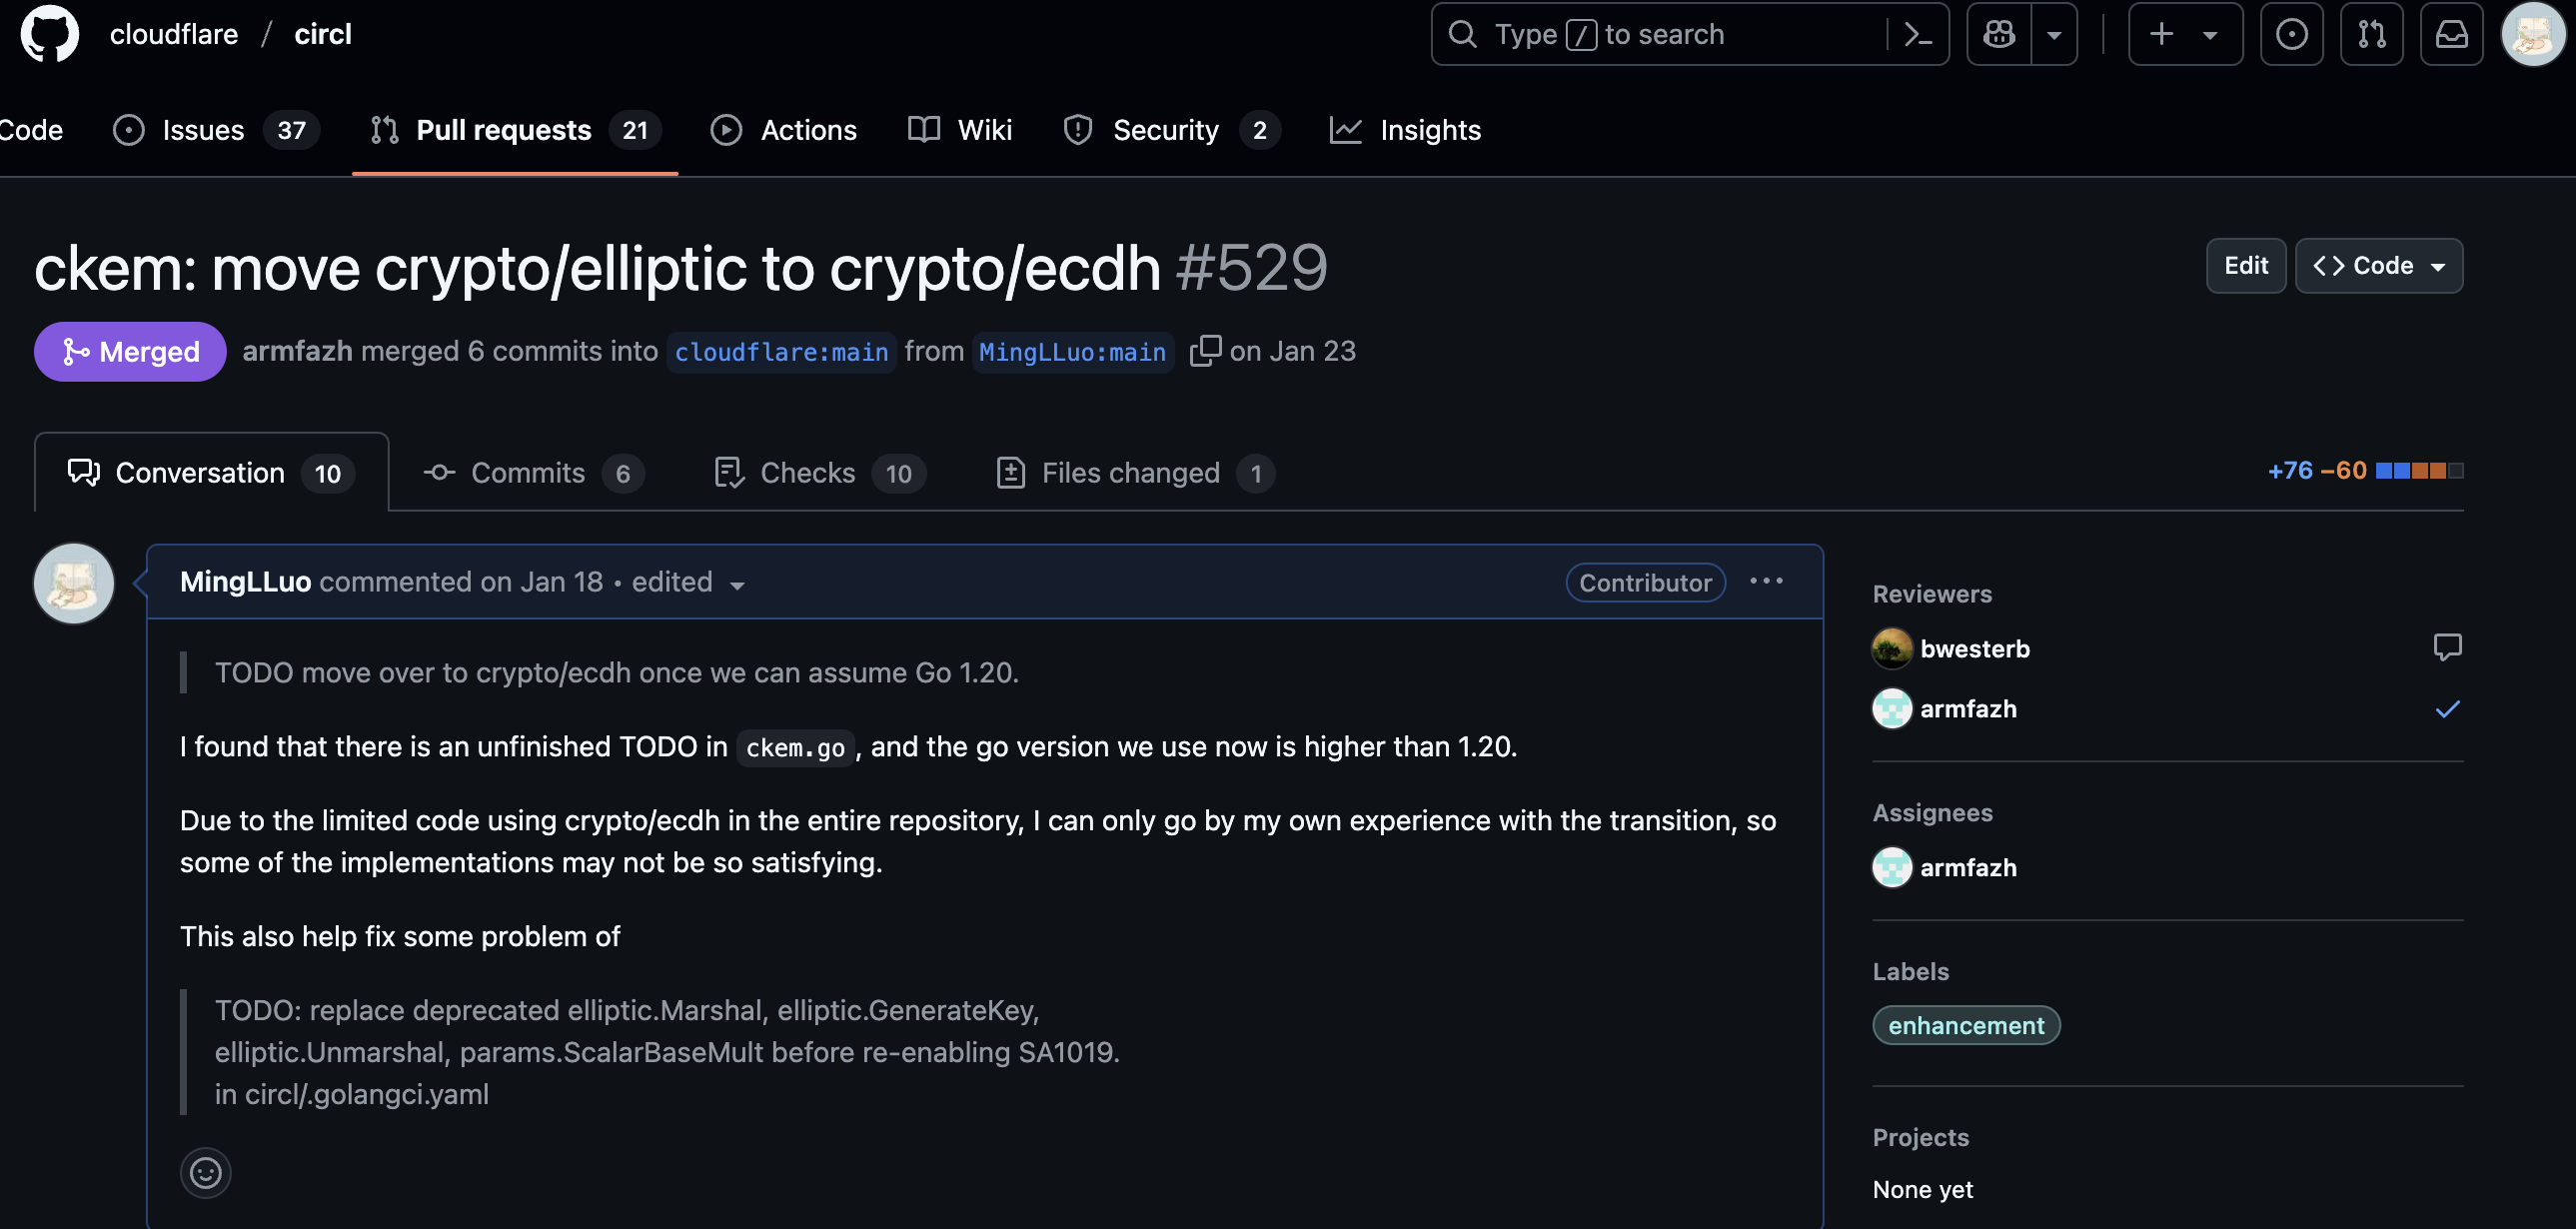
\includegraphics[width=0.85\textwidth]{figures/circl.png}
    \caption{Cloudflare CIRCL 库的开源贡献}
\end{figure}

\end{frame}

\section{致谢}
\begin{frame}
\frametitle{致谢}
\begin{center}
    \large 感谢评审老师们的耐心倾听!
\end{center}
\end{frame}

\end{document}